% GNUPLOT: LaTeX picture with Postscript
\begingroup
  \makeatletter
  \providecommand\color[2][]{%
    \GenericError{(gnuplot) \space\space\space\@spaces}{%
      Package color not loaded in conjunction with
      terminal option `colourtext'%
    }{See the gnuplot documentation for explanation.%
    }{Either use 'blacktext' in gnuplot or load the package
      color.sty in LaTeX.}%
    \renewcommand\color[2][]{}%
  }%
  \providecommand\includegraphics[2][]{%
    \GenericError{(gnuplot) \space\space\space\@spaces}{%
      Package graphicx or graphics not loaded%
    }{See the gnuplot documentation for explanation.%
    }{The gnuplot epslatex terminal needs graphicx.sty or graphics.sty.}%
    \renewcommand\includegraphics[2][]{}%
  }%
  \providecommand\rotatebox[2]{#2}%
  \@ifundefined{ifGPcolor}{%
    \newif\ifGPcolor
    \GPcolortrue
  }{}%
  \@ifundefined{ifGPblacktext}{%
    \newif\ifGPblacktext
    \GPblacktexttrue
  }{}%
  % define a \g@addto@macro without @ in the name:
  \let\gplgaddtomacro\g@addto@macro
  % define empty templates for all commands taking text:
  \gdef\gplbacktext{}%
  \gdef\gplfronttext{}%
  \makeatother
  \ifGPblacktext
    % no textcolor at all
    \def\colorrgb#1{}%
    \def\colorgray#1{}%
  \else
    % gray or color?
    \ifGPcolor
      \def\colorrgb#1{\color[rgb]{#1}}%
      \def\colorgray#1{\color[gray]{#1}}%
      \expandafter\def\csname LTw\endcsname{\color{white}}%
      \expandafter\def\csname LTb\endcsname{\color{black}}%
      \expandafter\def\csname LTa\endcsname{\color{black}}%
      \expandafter\def\csname LT0\endcsname{\color[rgb]{1,0,0}}%
      \expandafter\def\csname LT1\endcsname{\color[rgb]{0,1,0}}%
      \expandafter\def\csname LT2\endcsname{\color[rgb]{0,0,1}}%
      \expandafter\def\csname LT3\endcsname{\color[rgb]{1,0,1}}%
      \expandafter\def\csname LT4\endcsname{\color[rgb]{0,1,1}}%
      \expandafter\def\csname LT5\endcsname{\color[rgb]{1,1,0}}%
      \expandafter\def\csname LT6\endcsname{\color[rgb]{0,0,0}}%
      \expandafter\def\csname LT7\endcsname{\color[rgb]{1,0.3,0}}%
      \expandafter\def\csname LT8\endcsname{\color[rgb]{0.5,0.5,0.5}}%
    \else
      % gray
      \def\colorrgb#1{\color{black}}%
      \def\colorgray#1{\color[gray]{#1}}%
      \expandafter\def\csname LTw\endcsname{\color{white}}%
      \expandafter\def\csname LTb\endcsname{\color{black}}%
      \expandafter\def\csname LTa\endcsname{\color{black}}%
      \expandafter\def\csname LT0\endcsname{\color{black}}%
      \expandafter\def\csname LT1\endcsname{\color{black}}%
      \expandafter\def\csname LT2\endcsname{\color{black}}%
      \expandafter\def\csname LT3\endcsname{\color{black}}%
      \expandafter\def\csname LT4\endcsname{\color{black}}%
      \expandafter\def\csname LT5\endcsname{\color{black}}%
      \expandafter\def\csname LT6\endcsname{\color{black}}%
      \expandafter\def\csname LT7\endcsname{\color{black}}%
      \expandafter\def\csname LT8\endcsname{\color{black}}%
    \fi
  \fi
    \setlength{\unitlength}{0.0500bp}%
    \ifx\gptboxheight\undefined%
      \newlength{\gptboxheight}%
      \newlength{\gptboxwidth}%
      \newsavebox{\gptboxtext}%
    \fi%
    \setlength{\fboxrule}{0.5pt}%
    \setlength{\fboxsep}{1pt}%
\begin{picture}(7200.00,5040.00)%
    \gplgaddtomacro\gplbacktext{%
      \csname LTb\endcsname%
      \put(682,704){\makebox(0,0)[r]{\strut{}$0$}}%
      \put(682,1223){\makebox(0,0)[r]{\strut{}$5$}}%
      \put(682,1741){\makebox(0,0)[r]{\strut{}$10$}}%
      \put(682,2260){\makebox(0,0)[r]{\strut{}$15$}}%
      \put(682,2779){\makebox(0,0)[r]{\strut{}$20$}}%
      \put(682,3298){\makebox(0,0)[r]{\strut{}$25$}}%
      \put(682,3816){\makebox(0,0)[r]{\strut{}$30$}}%
      \put(682,4335){\makebox(0,0)[r]{\strut{}$35$}}%
      \put(814,484){\makebox(0,0){\strut{}$0$}}%
      \put(1544,484){\makebox(0,0){\strut{}$5$}}%
      \put(2274,484){\makebox(0,0){\strut{}$10$}}%
      \put(3004,484){\makebox(0,0){\strut{}$15$}}%
      \put(3733,484){\makebox(0,0){\strut{}$20$}}%
      \put(4463,484){\makebox(0,0){\strut{}$25$}}%
      \put(5193,484){\makebox(0,0){\strut{}$30$}}%
      \put(5923,484){\makebox(0,0){\strut{}$35$}}%
      \put(6055,704){\makebox(0,0)[l]{\strut{}$0$}}%
      \put(6055,1149){\makebox(0,0)[l]{\strut{}$0{,}5$}}%
      \put(6055,1593){\makebox(0,0)[l]{\strut{}$1$}}%
      \put(6055,2038){\makebox(0,0)[l]{\strut{}$1{,}5$}}%
      \put(6055,2483){\makebox(0,0)[l]{\strut{}$2$}}%
      \put(6055,2928){\makebox(0,0)[l]{\strut{}$2{,}5$}}%
      \put(6055,3372){\makebox(0,0)[l]{\strut{}$3$}}%
      \put(6055,3817){\makebox(0,0)[l]{\strut{}$3{,}5$}}%
      \put(6055,4262){\makebox(0,0)[l]{\strut{}$4$}}%
      \put(3354,4467){\rotatebox{90}{\makebox(0,0)[l]{\strut{}\footnotesize$\mathrm{K}_\alpha$}}}%
      \put(3675,4467){\rotatebox{90}{\makebox(0,0)[l]{\strut{}\footnotesize$\mathrm{K}_\beta$}}}%
    }%
    \gplgaddtomacro\gplfronttext{%
      \csname LTb\endcsname%
      \put(176,2519){\rotatebox{-270}{\makebox(0,0){\strut{}Ionisationsdosisleistung $\braket{j} / \si{\micro\ampere\per\kilogram}$}}}%
      \put(6692,2519){\rotatebox{-270}{\makebox(0,0){\strut{}Äquivalentdosisleistung $\dot{H} / \si{\sievert\per\hour}$}}}%
      \put(3368,154){\makebox(0,0){\strut{}Röhrenspannung $U / \si{kV}$}}%
      \csname LTb\endcsname%
      \put(2134,4162){\makebox(0,0)[r]{\strut{}Messdaten}}%
    }%
    \gplbacktext
    \put(0,0){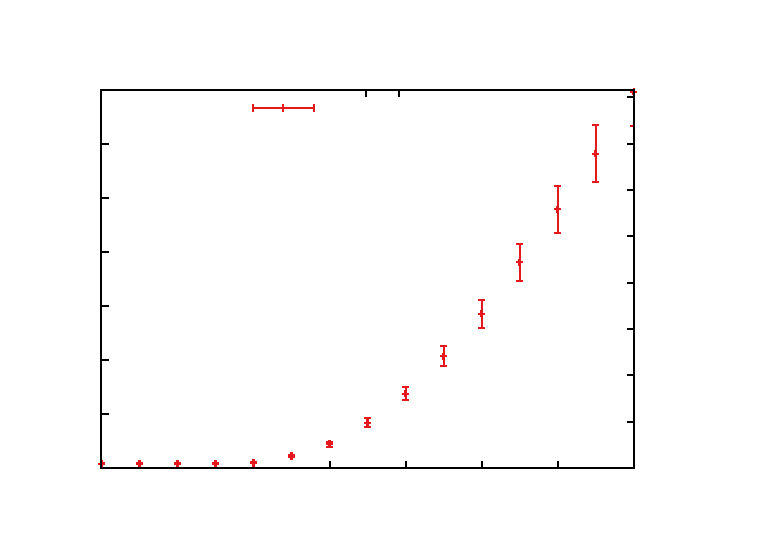
\includegraphics{./plots/dosis_roehrenspannung/mo}}%
    \gplfronttext
  \end{picture}%
\endgroup
